
The goal of this thesis is to identify resource intensive parts of a computer program which can be replaced by call to a semantically equivalent accelerator function with a lower execution time. 
\section{Problem definition}
To achieve our goals we first have to define what a \textit{part of a computer program} is. Therefore we have to know the language and structure of the input program. In this theses the input consists of \textit{LLVM IR}. This is an intermediate language which is used in the LLVM compiler framework. The advantage of an IR is the strict separation of compiler frontend, optimizer and backend. While the frontend can generate IR code from several source languages, the optimizer and backend only have to deal with a common intermediate language.


%TODO toolflow of llvm
The smallest organization unit of LLVM IR is an \textit{instruction}. LLVM IR uses Static single-assignment form (SSA) and three address code. Each instruction defines a variable with a unique name, which can be used multiple times. This introduces a \textit{def-use} chain, which we will use later to verify a valid replacement.

%TODO genauer ausführen?
Instructions are grouped into \textit{basic blocks}. Each basic block contains a maximal-length sequence of instructions that execute without a branch. Basic blocks are grouped into a \textit{function} where each function lives inside a \textit{module}. A module corresponds to a translation unit of the source language, e.g. a .c/.cpp-file.

All basic blocks of a function form a \textit{control-flow graph}(CFG). This is a directed graph $G=(V,E)$ where each node $n \in V$ corresponds to a basic block and each edge $(u,v) \in E$ represents a possible transfer of control (branch) from block $u$ to block $v$ \cite{cooper2012engineering}. An example of a simple control flow graph is illustrated in figure \ref{fig:cfgexample}.

\begin{figure}[htp] \centering{
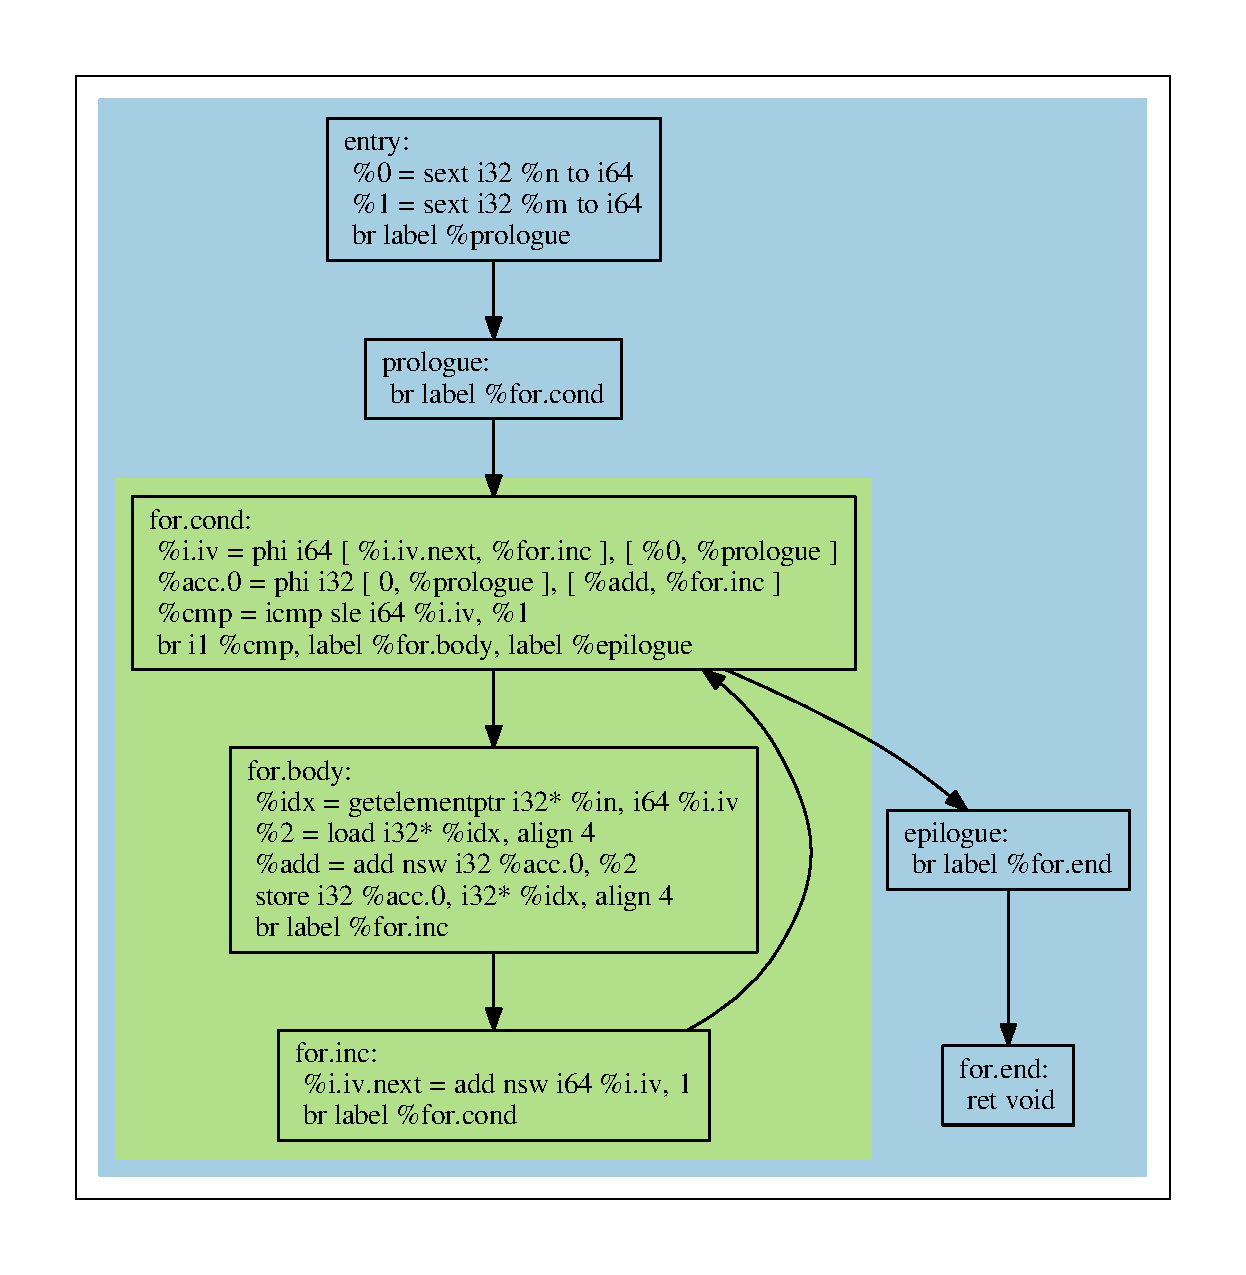
\includegraphics[scale=0.50]{figures/cfgexample.pdf}}
\caption{Example of a control-flow graph with basic blocks and their corresponding instructions.}
\label{fig:cfgexample}
\end{figure}

\begin{defn} Let $H$ be a subgraph of $G$, where $G$ is the complete control-flow graph of a function $F$. A part $P$ of a computer program, which is a candidate for replacement, is a subgraph $H$ consisting of as set of basic blocks. Each part $P$ has to suffice the following conditions:
\begin{itemize}
\label{def:program_part}

\item There exist at least one value in the successor blocks of $P$, argument list of $F$ or constant inside $P$ which is a used by $P$. These values are considered as \textit{input parameters}.
\item There exist zero or more instruction in $P$ that have an external users in one of the predecessor blocks of the induced graph $G/H$. These are considered as \textit{output parameters}.
%\item $H$ is a \textit{region} in $G$	%TODO: verifizieren, ob das im prototyp auch so ist: muss nicht so sein, da exit block schon wieder preheader z.B. für einen anderen block sein kann.
\end{itemize}

\end{defn}

In figure \ref{fig:cfgexample} this part, further referred to as \textit{candidate}, could be the set of basic blocks containing $C = \{for.cond, for.body, for.inc\}$, the input parameters $ \%0$ and $ \%1 $ and no output parameter. In this example they implement a simple loop. Epilogue and prologue are place holders for arbitrary code.

After defining what a valid candidate is, we also have to define what we mean by \textit{semantically equivalent}. We follow the definition in \cite{2000automatic} in a slightly modified form:

\begin{defn}
\label{def:sem_equiv}
Let $P$ and $P'$ be two program parts, where $P'$ is called a \textit{pattern} for $P$. Further let $I_i$ and $I'_i$ with $i = 0,\dots,n$ be the set of input parameters and $O_j$ and $O'_j$ with $j=0,\dots,m$ be the set of output parameters. 

$P$ and $P'$ are semantically equivalent if and only if they there is an binding of parameters with equal types with the $I_i = I'_j \quad \forall i,j \in 0 \dots n$ such that when $P'$ is called, one of the following is true:
\begin{itemize}
\item $P$ and $P'$ will not halt or
\item $O_i =O'_i \quad \forall i \in 0 \dots n$.
\end{itemize}
\end{defn}

In short definition \ref{def:sem_equiv} means: if two program parts have the same input, they always produce the same output. 
\\

We can now express the problem as followed: given an accelerator interface $A$, search a candidate $P$ and a binding of input parameters to $A$ such that they are semantically equivalent. Unfortunately there is no algorithm for testing the semantic equivalence of $P$ and $A$ since it is an undecidable problem.
\\

Instead of testing if $P$ is semantically equivalent to $A$, we only check if $P$ is an \textit{algorithmic equivalent} of $A$. Algorithmic equivalent was defined by Metzger et al. \cite{2000automatic}.

\begin{defn}
Let $P$ and $P'$ be two program parts. Define $P$ algorithmically equivalent to $P'$ ($P \equiv P'$)  if and only if one can be derived by another by the following operations:
\begin{itemize}
\item Simultaneous renaming of variables
\item Semantic preserving reordering of expressions
\item Permutation of commutative operations
\end{itemize}
\end{defn}

Listings \ref{lst:algeq_original_code} and \ref{lst:algeq_derived_code} showing an example of algorithmic equivalence. The right-hand side is derived from the left-hand side by renaming the variables in their declaration and use in both statements, exchanging the order in both statements (since there is not data dependency) and changing the operators in the multiplication statement.

\begin{figure}[!htb]
\noindent\begin{minipage}{.45\textwidth}
\begin{algorithm}[caption={Original code}, label=lst:algeq_original_code]
int i, j
float A[n][m], B[n][m]
for i = 2, i < n, i++
	for j = 2, j < m, j++
		A[i][j] = A[i][j-1]
		B[i-1][j-1] = 42 * B[i-2][j-2]
\end{algorithm}
\end{minipage}\hfill % no linebreak here
\begin{minipage}{.5\textwidth}
\begin{algorithm}[caption={Derived code}, label={lst:algeq_derived_code}]
int a, b
float X[r][t], Y[r][t] 
for a = 2, a < r, a++
	for b = 2, b < t, b++
		Y[a-1][b-1] = Y[a-2][b-2] * 42
		X[a][b] = X[a][b-1]
\end{algorithm}
\end{minipage}
\end{figure}

%TODO: beschreiben was ein induction value/variable ist, Variation von algorithmic instance
Metzger et al. also define the more general term of an \textit{algorithmic instance} which also covers the substitution of induction values. As our goal isn't to solve algorithmic recognition in general we will leave this definition by side.

\section{Algorithmic pattern recognition}

Our goal is to determine if there exist a \textit{candidate} in the input program which is algorithmically equivalent to the behaviour of one of our accelerator function. Therefore we require for each accelerator function one or more equivalent implementations. These implementations will be further referred to as \textit{patterns}. We will first take a look at pattern representation in section \ref{sec:pattern_representation}.

Of course there is a potential for slight variations in the input program. If we take a look at the statement level there are multiple ways to represent an arithmetic expression. E.g. $a = b *( c + d ) \equiv a = b*c + b*d$. These variations also exist on the control-flow level. In order to reduce the number variations in the input we first have to canonicalize it. LLVM provides a brought range of canonicalization passes, which we will revise in section \ref{sec:program caninicalization}

To check if one of our patterns is included in the input, we first have to check whether there exists a subgraph in the input control-flow graph which can be mapped to one of our patterns. This problem is known as \textit{subgraph isomorphism}. The isomorphism gives us a injective mapping of nodes from the candidate CFG to the pattern CFG. We will later see a formal definition of a subgraph isomorphism, common algorithms to find them and an examples in section \ref{sec:control_flow_matching}.

If we found a mapping from the pattern control-flow to a possible candidate, we have to check if this assignment is valid. For each potential transfer of control the branch has to happen under the same condition as in the pattern. Further we have to check for each expression in the pattern if there exist a corresponding expression in the candidate. We will deal with this problem in section \ref{sec:matching_statements}.

\subsection{Pattern representation}
\label{sec:pattern_representation}
%How are patterns represented in my toolchain, and why are they represented in that way?
%TODO: Prüfen, ob überall control flow statt control-flow geschrieben wurde
A pattern includes the required control-flow of basic blocks, the condition for each possible transfer of control and all computational statements. Additionally a pattern includes which hardware interface is represented. For an interface a pattern also defines what values  of the statements were bound to which argument. All information are encoded in the \textit{JavaScript Object Notation} (JSON) format. JSON is an open, text based, human-readable data interchange format with a small set of formatting rules \ref{bib:rfcjson}. Although patterns can be generated from llvm functions, the specific binding to an interface can not be automatically derived. The properties of JSON, in particular the human-readability, facilitate the postprocessing of patterns.

A set of patterns can be combined to form a database. %TODO hier ausführen

\begin{formatdesc}[mathescape, caption={Pattern format description}, label={lst:patternformat}]

Pattern	:= '{' VersionAttr ',' NameAttr ',' HWIface ',' Graph '}'

HWIface	:= 'hwiface:' '{' NameAttr Binding '}'
Binding	:= 'binding:' '[' ('[' $int$, $llvmtype$']' Sep )+ ']'

Graph	:= 'graph:' '{' '[' NodeObj ',' EdgeObj ']' '}'
NodeObj	:= '{' 'nodes:' '[' (Node Sep)+ ']' '}'
EdgeObj	:= '{' 'edges:' '[' (Edge Sep)+ ']' '}'
Edge	:= '{' 'src:' $int$, 'dst': $int$ '}'

Node	:= '{' IDAttr ',' Attributes  '}'

Attributes	:= 'attributes:' '{' (CFGAttributes | StmtAttributes) '}'

CFGAttributes	:= LabelAttr? ExpressionsAttr?
StmtAttributes	:= 
				'{' (OpcodeAttr | ArgAttr | ConstAttr) ','
					IValAttr? ',' TypeAttr	'}'

ExpressionsAttr := '[' Graph+ ']'

VersionAttr	:= 'version:' $int$
NameAttr	:= 'name:' $string$
IDAttr		:= '_id:' $int$
OpcodeAttr	:= 'opcode:' '['  ']'
ArgAttr		:=  'argument:' $string$
ConstAttr	:=  'const' ($int$ | $float$ | $double$)
TypeAttr	:= 'type:' $llvmtype$
IValAttr	:= 'i_val:' [$int$, $int$, $string$]
LabelAttr	:= 'labels:' '[' ($int$ Sep)+ ']'

Sep := ',' | $\epsilon$
\end{formatdesc}

Due to the text based nature of JSON, one major drawback is the size of a pattern as file. They become large even for relative simple program parts. An instance of the format \ref{lst:patternformat} can be found in appendix \ref{anhangPattern}.

\subsection{Program canonicalization}
\label{sec:program caninicalization}

%Which passes are required to canonicalize an input program

There are several ways to write down an abstract operation like convolution in a high-level language like C. Besides the fact that there are several algorithms, each algorithm can be expressed in a different way. Similar formulations with minor differences in the high level language can in turn produce different outcomes in LLVM IR. E.g. computational statements like $x = 8 * ( a + b )$ can be expressed as $x = 8*a + 8*b$ or $x = a << 3 + b << 3$ and so on. Although these variations can also be covered by increasing the number of patterns, the recognition process will be faster if the number of patterns is small. One idea to reduce the number of variations is to transform the program into a \textit{canonical} form as suggested in \cite{2000automatic}.

In order to canonicalization the LLVM IR, one can make use of the already available transformation passes, implemented in the optimizer. There are several passes that can be used for normalization. In the following we will look at some of LLVMs optimizations which we can use for canonicalization.

\subsubsection{Interprocedual canonicalization}
%TODO beschreiben, dass er es nicht tut und warum
As our recognition pass does not look across a functions boundary we have to inline eventually called functions. This is accomplished by using llvms inlining pass. In practice the inliner calculates the \textit{costs} for each potential inlining. A threshold then decides whether the callee gets inlined  or not. The costs are calculated based on the number of arguments, their method of passing, the number and type of instructions and so on. Thus the number of patterns we can recognize also depends on the inlining costs, which can be given as an input to the optimizer. As we will see in the evaluation the default cost threshold of 255 turn out to be valid trade-off.

Why inlining is required is illustrated in figure \ref{alg:inline_opportunity}. Even if one can recognize that the \textit{matrix\_multiply($\dots$)} is candidate for hardware migration, the speedup would be rather small, as the matrices in image processing are usually $3x3$ or $4x4$. However if we inline this operation and involve the two other loops, we may gain a speedup.

\begin{algorithm}[mathescape, caption={Potential inlining opportunity}, label={alg:inline_opportunity}]
for (j = 0; j < ny; ++j){
	for (i = 0; i < nx; ++i) {
	$\dots$
	matrix_multiply($\dots$)
	$\dots$
	}
}
\end{algorithm}

\subsubsection{Control flow canonicalization}

A critical part of the control-flow are loops. LLVM detects natural loops using the \textit{loop} analysis pass. A natural loop has exactly one entry point, the \textit{header} block, which dominates all blocks in the loop. The header has exactly one \textit{backedge} entering it. A backedge is an edge coming from one block of the loop body \cite[p.662-665]{aho2014compilers}. \\

The first transformation pass we apply is the \textit{loop-simplify} pass. This pass guarantees that the resulting loop has the following properties:
\begin{itemize}
\item The header block has a single, non-critical input edge coming from a \textit{pre-header} block outside the loop.
\item A loop must have a \textit{latch}, the source node of the only backedge. This block will be executed in before every new iteration. The latch is not required to be a separate block. It can be the same block as the header.
\item There is a single exit block which will always be executed after loop exit.
\end{itemize}

Loop invariant code motion (\textit{licm}) is another optimization pass which contributes to canonicalization. This pass tries to move as much invariant instructions as possible from inside of a loop body to its pre-header or exit block. Thus moving expression which have the same value at each iteration out of the loop.\\

\noindent\begin{minipage}{.45\textwidth}
\begin{algorithm}[caption={Before licm}]
for (j = 0; j < n; ++j)
	for (i = 0; i < m; ++i) {
		a = b + c
		C[j][i] = a
	}
\end{algorithm}
\end{minipage}\hfill % no linebreak here
\begin{minipage}{.5\textwidth}
\begin{algorithm}[caption={After licm}]
a = b + c
for (j = 0; j < n; ++j)
	for (i = 0; i < m; ++i) {	
	 C[j][i] = a
	}
\end{algorithm}
\end{minipage}

Loop unrolling is a well known optimization technique, however it makes algorithm recognition difficult. When the iteration count of a loop is known at compile time the compiler may replicate the loop body as many times as the loop gets iterated and builds instances of the induction values where they were used \cite[p. 441]{cooper2012engineering}. However this requires to have a pattern for each potential unrolling count. In order to reduce the number of patterns Metzger et. al \cite{2000automatic} suggest to re-roll the loops. However there is currently not general loop-rerolling pass in llvm. Thus we will only recognize program parts which were not unrolled.

\subsubsection{Basic Block canonicalization}

There are several optimizations that work in the scope of one basic block. In the following we list the most common.

\begin{description}
\item Memory to register (mem2reg)\\
switch: -mem2reg\\\\
This pass promotes alloca instruction into scalar registers (SSA values). Load and store instructions are replaced by register access. This enables a set of further optimizations.

\begin{minipage}{.45\textwidth}
\begin{llvmcode}[mathescape, caption={Before mem2reg}]
define i32 @foo(i32 %n) {
entry:
  %n.addr = alloca i32, align 4
  store i32 %n, i32* %n.addr, align 4
  br label %some_bb

some_bb:
  %0 = load i32* %n.addr, align 4
  %1 = add i32 %0, 1
$\dots$
\end{llvmcode}
\end{minipage}\hfill % no linebreak here
\begin{minipage}{.5\textwidth}
\begin{llvmcode}[mathescape, caption={After mem2reg}]
define i32 @foo(i32 %n) {
entry:
  br label %some_bb

some_bb:
  %1 = add i32 %n, 1
   
 
 
$\dots$
\end{llvmcode}
\end{minipage}

\item Combining redundant instructions\\
switch: -instcombine\\\\
This pass combines redundant instructions to generate fewer instruction in the output llvm code. There is also canonicalization performed, e.g. all constant operands were moved to the right hand side, multiplications with power of two arguments are translated to shifts, and so on. The full list is provided in \cite{bib:llvm_passes}.

\begin{minipage}{.45\textwidth}
\begin{llvmcode}[mathescape, caption={Before instcombine}]
%1 = add i32 %0, 5
%2 = add i32 %1, 3
$\dots$
\end{llvmcode}
\end{minipage}\hfill % no linebreak here
\begin{minipage}{.5\textwidth}
\begin{llvmcode}[mathescape, caption={After instcombine}]
%2 = add i32 %0, 8

$\dots$
\end{llvmcode}
\end{minipage}

\item Common subexpression elimination\\
switch: -early-cse\\\\
A common subexpression is a part of an expression which has been previously computed. E.g. $y = n*11 +( m + (n*11))$ can be reduced to $x = n * 11$ and $y = x + (m + x)$. This opens an opportunity for further reductions such, e.g. $y = 2 * x + m $ where strength reduction can be applied: $y = x << 2 + m$.

Early common subexpression elimination removes these trivially redundant instructions in an early stage of the optimization.

\begin{minipage}{.45\textwidth}
\begin{llvmcode}[mathescape, caption={Before early-cse}]
%n1 = load i32* n, align 4	; readonly
%1 = add i32 %n1, 5
%n2 = load i32* n, align 4  ; readonly
%2 = add i32 %n2, 0
%3 = mul i32 %2, 3
$\dots$
\end{llvmcode}
\end{minipage}\hfill % no linebreak here
\begin{minipage}{.5\textwidth}
\begin{llvmcode}[mathescape, caption={After early-cse}]
%n1 = load i32* n, align 4	; readonly
%1 = add i32 %n1, 5
%3 = mul i32 %n1, 3


$\dots$
\end{llvmcode}
\end{minipage}

\item Reassociates commutative expressions\\
switch: -reassociate \\\\
This pass reassociates commutative expression. E.g. $a = (x + 4) + 9$ will be transformed into $a = x + (4 + 9)$. A subsequent pass constant propagation, or instcombine pass will lower this expression into $a = x + 13$.
\end{description}


\subsection{Matching the control flow}
\label{sec:control_flow_matching}
%General description of graph matching problem in context of LLVM. And specific description of two famous algorithms (with fancy graphics)

As mentioned in the overview of this section, matching the control-flow of a possible candidate to the pattern control-flow, is the problem of finding the subgraph isomorphism of two graphs. First, we formally define what a subgraph isomorphism is, afterwards we revise a well known algorithms to solve this task in practice.

\begin{defn}
\label{def:subgraph_iso}
Let $G=(V, E)$ and $H=(V', E')$ be two graphs. A subgraph isomorphism of $H$ into $G$ is an injective relation $A\subseteq V \times V'$ such that for every pair $(v_i, v_j) \in V'$ and $(w_i, w_j) \in V$ with $(v_i, w_i) \in A$ and $(v_j, w_j) \in A$, $(w_i, w_j) \in E$ if $(v_i, v_j) \in E'$. $A$ is then called the subgraph isomorphism of $H$ in $G$ \cite{valiente2002algorithms}.
\end{defn}

Figure \ref{fig:subgraphisoexample} illustrates the subgraph isomorphism of two graphs. Checking whether two graphs are isomorphic to another is not known to be in P or NP. The program is a special case of the general subgraph isomorphism, which is an NP-complete problem \cite{wegener2005complexity}.

\begin{figure}[!htb]
\begin{tikzpicture}[remember picture]
  \node (G) {
  	\begin{tikzpicture}[main node/.style={circle,draw,minimum size=.8cm,inner sep=0pt}]
		\node[main node] (G1) {$a$};
		\node[main node] (G2) [right = 1cm of G1] {$b$};
		\node[main node] (G3) [right = 1cm of G2] {$c$};
		\node[main node] (G4) [right = 1cm of G3] {$d$};
		\node[main node] (G5) [right = 1cm of G4] {$e$};
		\node[main node] (G6) [below = 1.5cm of G2] {$f$};
		\node[main node] (G7) [below = 1.5cm of G3] {$g$};
		
		\path[draw,thick]
		(G1) edge node {} (G2)
		(G2) edge node {} (G3)
		(G3) edge node {} (G4)
		(G4) edge node {} (G5)
		(G2) edge node {} (G6)
		(G3) edge node {} (G7)
		(G6) edge node {} (G7)
		(G4) edge [bend right=50] node {} (G2);
  	\end{tikzpicture}
  };
	\node at (0,-2.5) {Graph G};
    %%
    \node(H)[right=of G]{
	\begin{tikzpicture}[main node/.style={circle,draw,minimum size=.8cm,inner sep=0pt}]
    \node[main node] (H1) {$1$};
    \node[main node] (H2) [right = 1cm  of H1]  {$2$};
    \node[main node] (H3) [right = 1cm  of H2] {$3$};
    \node[main node] (H4) [right = 1cm  of H3] {$4$};

    \path[draw,thick]
     (H1) edge node {} (H2)
     (H2) edge node {} (H3)
     (H3) edge node {} (H4)
     (H1) edge [bend left=50] node {} (H3)
    ;
    \end{tikzpicture}   
    };   
    \node at (8, -2.5) {Graph H};
    \path[draw,dashed]
    	(H1) edge [bend right=80, ->] node {} (G2)
    	(H2) edge [bend right=80, ->] node {} (G3)
    	(H3) edge [bend right=80, ->] node {} (G4)
    	(H4) edge [bend right=80, ->] node {} (G5)
    ;
\end{tikzpicture}
\caption{Example of a subgraph isomorphism}
\label{fig:subgraphisoexample}
\end{figure}

Since finding a subgraph isomorphism is required in a wide range of disciplines, from chemistry to circuit design, there exist a couple of algorithms to cope with this task. They usually give a lower bound for the runtime and perform quite good on graphs with a small number of nodes. The number of nodes in control-flow graphs is in practice usually not as large as it would produce a huge runtime for isomorphism-algorithms. However this statement does not hold for all input programs. We have to keep in mind that finding an isomorphism might have exponential runtime.

\subsubsection{Ullmann}

% TODO schreiben warum hier ullmann verwendet wurde

A naive algorithm would enumerate all possible assignments of nodes from $H$ to nodes of $G$ and check for each assignment whether it is valid, according to the edge sets of both graphs. It is obvious that the search space becomes exponential in the number of nodes.

A more efficient algorithms for subgraph isomorphism was invented by Ullmann \cite{Ullmann:1976} in 1976. His algorithm extends the naive approach by continually removing infeasible assignments using a \textit{refine procedure}. This narrows the search space and therefore reduces the runtime.

The original algorithm introduced by Ullmann in intended to work with adjacent matrices of undirected graphs, however our input looks different. The input, as illustrated in figure \ref{fig:cfgexample}, is a directed graph, where each node only knows its successor nodes. Thus we will translate the original algorithm to work directed graphs an adjacent lists such that we can find a subgraph isomorphism of a given pattern control-flow $H$ in the input control-flow $G$.

In the implementation we made use of the \textit{graph-traits} concepts of LLVM. This will make our algorithms work with arbitrary graphs, not only control-flow graphs. Graph-traits can be thought of as a generalized interface for graphs, which decouples their actual representation from algorithms which work on them. %TODO satz checken
\\

%TODO narrow function beschreiben
Like Ullmanns algorithm, procedure $calculate\_possible\_assignments(\dots)$ (listing \ref{alg:calculate_possible_assignments}) first calculates all possible assignment from the nodes of $V'$ of $H$ to the nodes $V$ of $G$, which we denote as the function $P$. For each node $u \in V'$ this is the set $V'' = \{\quad v \in V\quad |\quad\forall u \in V': deg(v) \geq deg(u) \land nfn(u, v)\}$ where $nfn(\dots)$ is an additional narrow function. This function will further thin out the number of possible assignments in order to speed up our matching process. Figure \ref{fig:possibleassignment_example} illustrates this operation for an exemplary control-flow.
\begin{algorithm}[mathescape, caption={Find isomorphism}, label={alg:find_isomorphism}]
find_isomorphism(GraphT G, GraphT H, list<map<NodeT* NodeT*>> A, nfn(NodeT*,NodeT*)) -> bool

    map<NodeT*, set<NodeT*>> P
    calculate_possible_assignments(G, H, P, nfn)
    found_assignment $\gets$ true
    while(found_assignment)    
        found_assignment $\gets$ false
        map<NodeT*, NodeT*> tmp
            
        if(recursive_find_isomorphism(G, H, P, tmp))
   	        A.add(tmp)
            found_assignment $\gets$ true;
            foreach(pair p : tmp)
                NodeT* Y $\gets$ p.first
                NodeT* X $\gets$ p.second
                P[Y].remove(X)	// Remove assigned node to find no isomorphism twice
                
\end{algorithm}


\begin{figure}[!htb]
\begin{minipage}{0.5\textwidth}  
\begin{tikzpicture}[remember picture,baseline=0]
%%
  \node (G) {
   
   \begin{tikzpicture}[main node/.style={circle,draw,minimum size=.8cm,inner sep=0pt}]
  	
	 \path   (0, 0)  node[main node]  (2) {$a$}
	         (2, 0)  node[main node]  (3) {$b$}
	         (1, -2)  node[main node] (4) {$c$}
	         (0, -4)  node[main node] (5) {$d$}
			 (2, -4)  node[main node] (6) {$e$}
			 (1, -6)  node[main node] (7) {$f$}
			 (-1, -2)  node[main node] (8) {$g$};

	\path[->, thick]
			(2) edge node {} (4)
			(2) edge node {} (8)
			(8) edge node {} (5)
			(3) edge node {} (4)
			(4) edge node {} (5)
			(4) edge node {} (6)
			(5) edge node {} (7)
			(6) edge[bend right] node {} (4)
			(6) edge node {} (7);
		
	\draw[->, dashed] (0,1) to node {} (2);
	\draw[->, dashed] (2,1) to node {} (3);
	\draw[->, dashed] (7) to node {} (0, -7);
	\draw[->, dashed] (7) to node {} (2, -7);

    \draw (0,-8) node {$G$};
  	\end{tikzpicture}
  };

    %%
    \node(H)[right=of G]{
	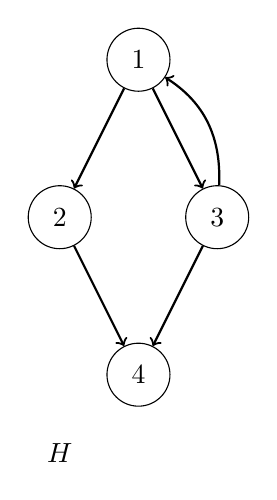
\begin{tikzpicture}[main node/.style={circle,draw,minimum size=.8cm,inner sep=0pt}]
  	 \path   (1, -2)  node[main node] (4) {$1$}
  	         (0, -4)  node[main node] (5) {$2$}
  			 (2, -4)  node[main node] (6) {$3$}
  			 (1, -6)  node[main node] (7) {$4$};
  
  	\path[->, thick]
  			(4) edge node {} (5)
  			(4) edge node {} (6)
  			(5) edge node {} (7)
  			(6) edge[bend right] node {} (4)
  			(6) edge node {} (7);
    \draw (0,-7) node {$H$};
    \end{tikzpicture}   
    };
\end{tikzpicture}
\end{minipage}\hfill
\begin{minipage}{0.5\textwidth}
Let $H=(V',E')$ and $G=(V,E)$ then a possible assignments is a function $P: V' \to V''$
\begin{itemize}
\item $P(1) =\{c, e, f,\dots\} $
\item $P(2) =\{a, b, c, d, g,\dots \} $
\item $P(3) =\{c, e,\dots\} $
\item $P(4) =\{c, f,\dots\} $
\end{itemize}
\end{minipage}
\caption{Possible assignments for a subgraph.}
\label{fig:possibleassignment_example}
\end{figure}


\begin{algorithm}[mathescape, caption={Calculate possible assignments}, label={alg:calculate_possible_assignments}]
calculate_possible_assignments(GraphT G, GraphT H, map<NodeT*, set<NodeT*>> P, nfn(NodeT*,NodeT*)) -> void

    foreach(NodeT* u : H)
    	set<NodeT*> candidates
        foreach(NodeT* v : G)        
            if(deg(v) $\geq$ deg(u) and nfn(u,v))
                candidates.add(v);
	    P.add((N, candidates))
\end{algorithm}


After calculating possible assignments the algorithm uses $recursive\_find\_isomorphism(\dots)$ to recursively test each possible assignments. Line 4-9 in listing \ref{alg:recursive_find_isomorphism} test whether an assignment is feasible. Referring to definition \ref{def:subgraph_iso} an assignment is feasible if and only if for each edge $(v_i,v_j)$ in the subgraph $H$ there is also an edge $(A(v_i),A(v_j))$ in $G$. In other words, for each edge in $H$ there must be corresponding edge in $G$. If an assignment is not feasible the algorithm returns false and another path in the search tree will be taken.

Let $A$ be an assignment in the example of figure \ref{fig:possibleassignment_example} with $A(1) = e$, $A(2) = b$ and so on. $A$ is not a feasible, because $(e, b) \notin E$.

\begin{algorithm}[mathescape, caption={Recursive find isomorphism}, label={alg:recursive_find_isomorphism}]
recursive_find_isomorphism(GraphT G, GraphT H, map<NodeT*,set<NodeT*>> P, map<NodeT*,NodeT*> A) -> bool
    
    refine_assignments(P);
    foreach(NodeT* uH : H)
        foreach(NodeT* vH : children(u))
            NodeT* uG $\gets$ A[uH]
            NodeT* vG $\gets$ A[vH]
            if(!is_edge(uG, vG)) // check if (uG, vG) is an edge in G
                return false

    if($\abs{A} == \abs{H}$)
        return true
    
    foreach(NodeT* Y : H)    
        if(A.contains(Y))  // skip node if already assigned
            continue    	
        set<NodeT*> candidates = P[Y];        
        foreach(NodeT* X : candidates)            
            A.add((Y, X))
            map<NodeT*, set<NodeT*>> $P'$ $\gets$ P.copy()
            // update_possible_assignments(...)
            // Removes a node X from all possible assignments, except for Y
            update_possible_assignments(Y, X, $P'$) 
            if(recursive_find_isomorphism(G, H, $P'$, A))
                return true            
            A.remove((Y,X))
    return false
\end{algorithm}


The actual speedup comes from Ullmanns refinement procedure which is implemented in the $refine\_assignments(\dots)$ function. The function checks for each node $u \in V'$ and each possible assignment $v = P(u)$ if there is least one neighbour $u' = children(u)$ is in the set $P(v')$, where $v' = children(v)$. This check will be executed until no further deletions are possible.


\begin{algorithm}[mathescape, caption={Refine possible assignments}, label={alg:refine_assignments}]
refine_assignments(map<NodeT*, set<NodeT*>> P) -> void
    changes $\gets$ true
    while(changes)
        changes $\gets$ false
        foreach(pair p : P)
             NodeT* Y = p.first
             set<NodeT*> candidates = p.second
             
             foreach(NodeT* X : candidates)
                 match $\gets$ true if #children(Y) == 0 otherwise false 
                 
                 foreach(NodeT* ny : children(Y)) // neighbour of Y
                     set<NodeT*> A $\gets$ P[ny]
                     foreach(NodeT* nx : children(X)) // neighbour of X
                         if(A.contains(nx))
                             match $\gets$ true
                 if(!match)
                     candidates.remove(X)
                     changes $\gets$ true
\end{algorithm}

Let us again consider the example in figure \ref{fig:possibleassignment_example} and look at the assignment $P(2) = g$. Node $4$ is a neighbour of $2$, but none of the neighbours of $g$ (which is $d$) is in the set of possible assignments of $4$. Thus the assignment $2 \rightarrow g$ will never be possible and $g$ will be removed from the set $P(2)$.

If an assignment is feasible and all nodes of $H$ were assigned, the recursive function finally returns true. Because there might be multiple subgraph isomorphisms the function $find\_isomorphism(\dots)$ will delete the previous found assignment from the possible assignments and will search again, until no more isomorphisms were found.

The more is known about the nodes the further we can restrict number of possible assignments before running the algorithm. Hence some nodes are associated with one or more \textit{labels}. The label describes a role in the control-flow. Possible labels are \textit{entry}, \textit{exit}, \textit{loop\_header}, \textit{loop\_inc}, \textit{loop\_body} and so on. A node with a \textit{loop\_inc} label can never be mapped to a \textit{entry} node.

%TODO \subsubsection{VF and VF2} muss das wirklich sein?

\subsection{Matching Statements}
\label{sec:matching_statements}

In the previous section we showed that it is possible to find a control-flow in the input which is equal to one of our patterns control-flow. Now we have to check if the assignment is valid, according the branch conditions and computations carried out by the nodes of the input CFG with respect to our pattern.

As described in \ref{sec:pattern_representation} each node is associated with a list of statements. Since we only consider programs of a restricted domain we look at statements which are either a branch expression or a expressions which sink in a store instruction.

\begin{figure}[htp] \centering{
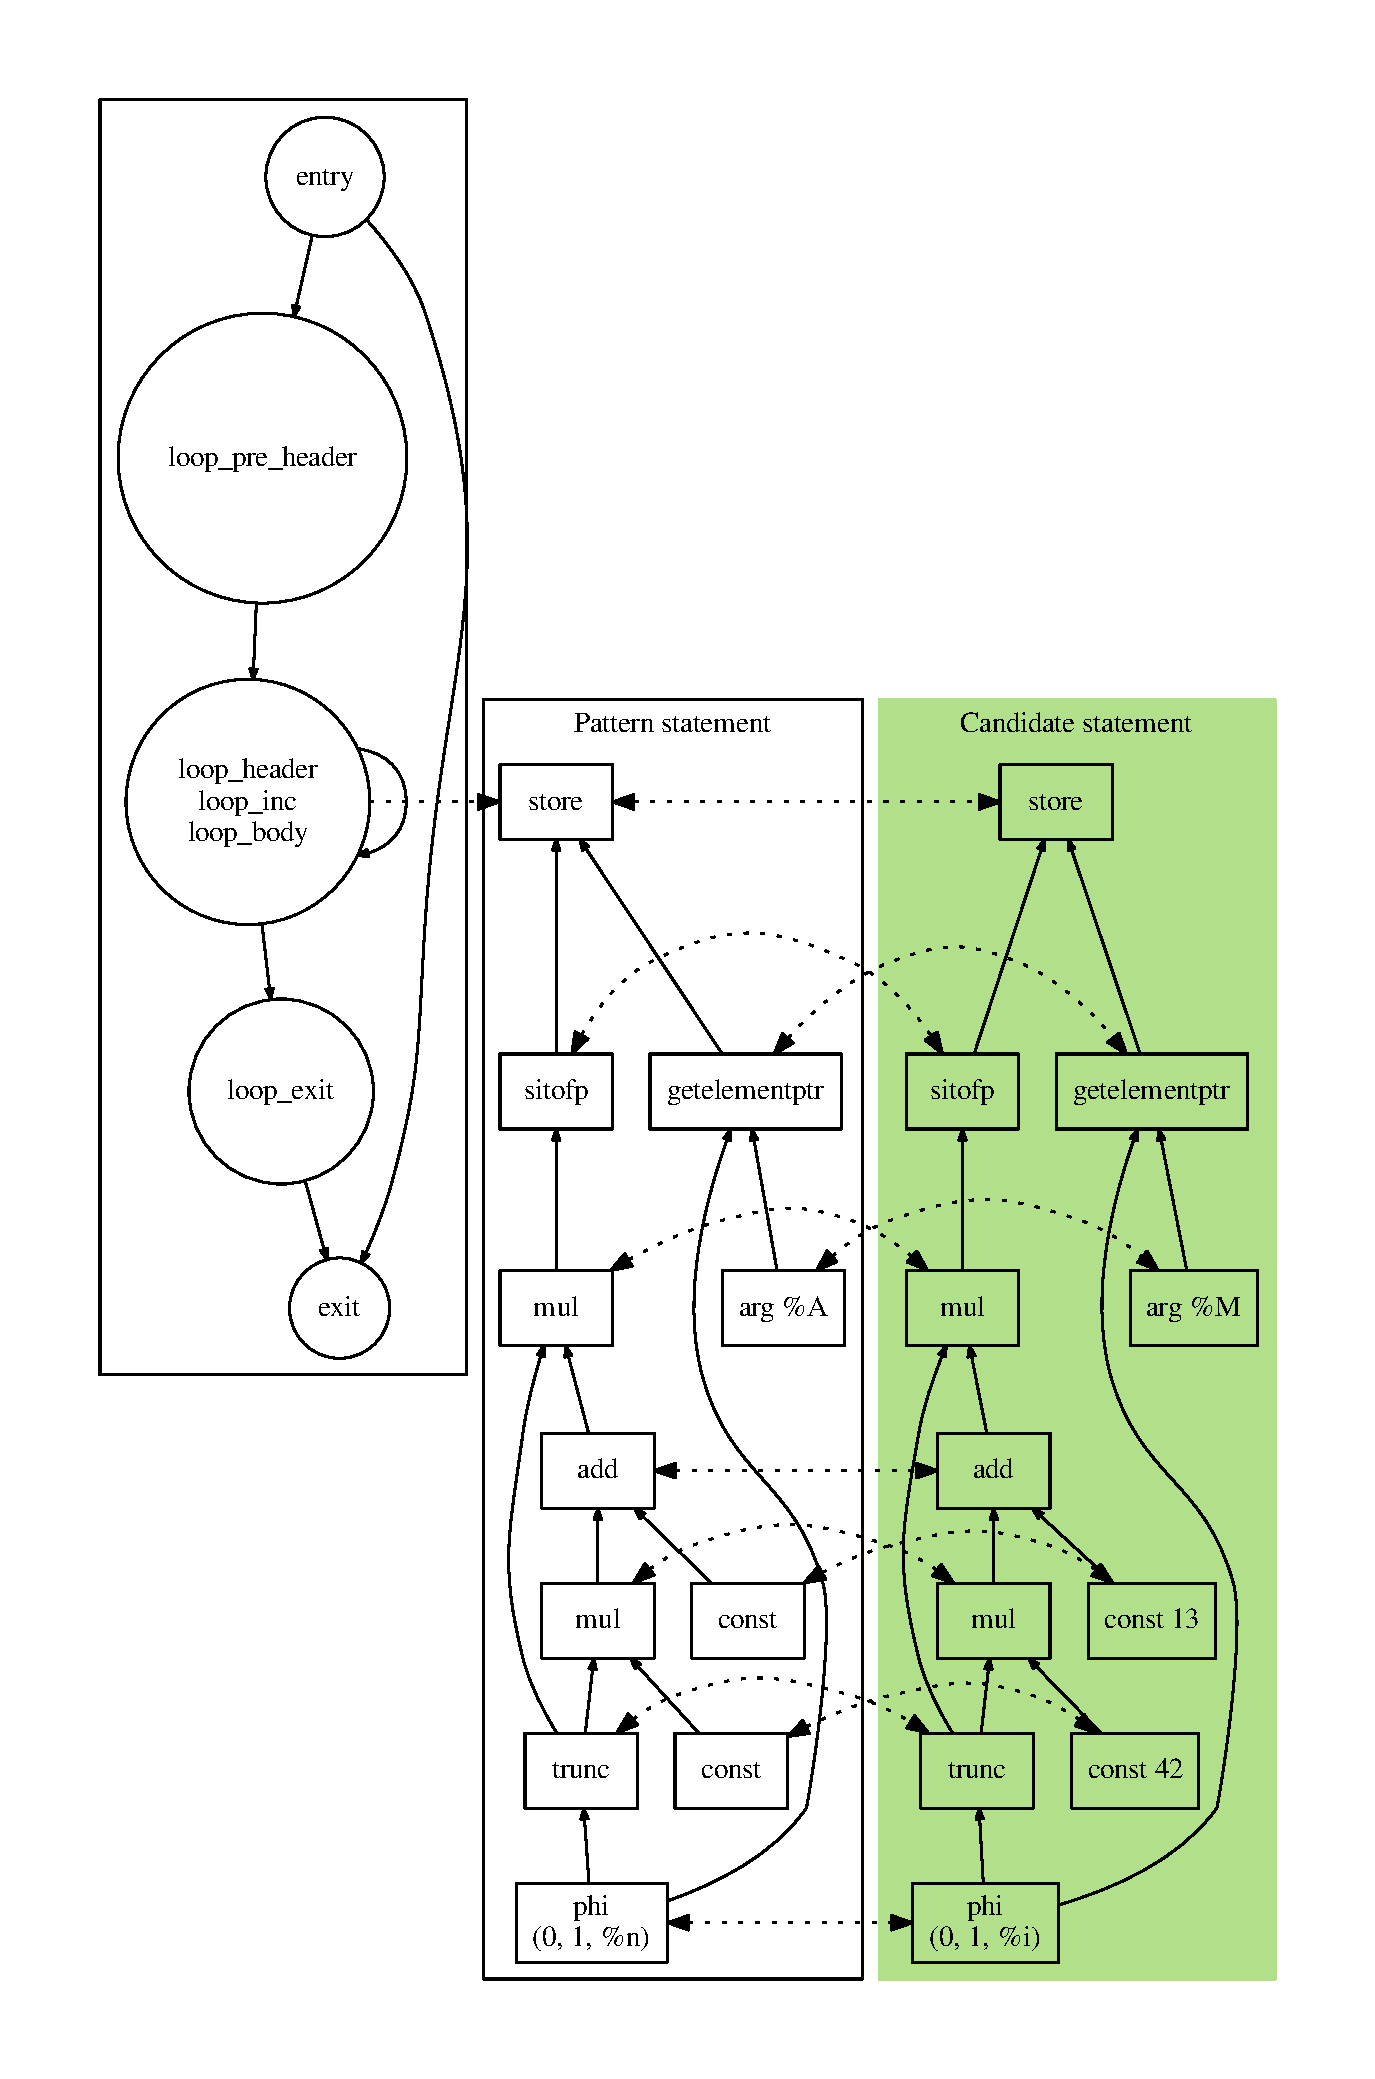
\includegraphics[scale=0.5]{figures/graphs/dot/foo.dot.pdf}}
\label{fig:abstractCFGOfFoo}
\caption{Abstract control-flow graph for the pattern of function \textit{foo}.}
\end{figure}

From \ref{sec:program caninicalization} we known that each statement consists of a canonicalized directed acyclic graph (DAG). Each node of the DAG (in the figure \ref{fig:abstractCFGOfFoo} represented as a rectangular) represents an instruction carried out by a statement.

To finally match a statement from our pattern to a statement of a candidate we have to traverse both DAGs simultaneously in depth-first order to compare whether each value suffice the following conditions:
\begin{itemize}
\item Each instruction from the pattern statement has the same opcode as the candidate instruction.
\item For each induction variable (IV), aka phi-node, in the pattern the \textit{start}, \textit{step} and \textit{exit} expression is equal to the candidate IV.
\item The resulting data type of each value in the candidate statement is the same as the data type of our pattern value.
\end{itemize}

%TODO paramters von hw interface beschreiben
For each value of the pattern statement we establish a bidirectional mapping to the matched value in the candidate statement. Thus we know which constant or function argument, (which are the input values of the hardware interface) is bound to the corresponding value in the candidate statement (and vice versa). We will use these bindings in section \ref{sec:hw_iface_binding} in order to bypass the input parameters of the matched program part to the hardware interface. This binding is illustrated in figure \ref{fig:abstractCFGOfFoo} using the dotted bidirectional arrows between both statements.

\section{Pattern extraction}

In this section we will describe how a recognized algorithm can bound to a hardware interface. In general it doesn't matter what particular accelerator lives behind an interface, whether its a GPU or an FPGA. In this thesis we use the Maxeler dataflow computer as our main platform, thus in our case an FPGA lives behind the interface \ref{sec:maxeler}.

%\subsubsection{Overlays}
%First we will describe which particular accelerators we use

\subsubsection{Binding a program part to a hardware interface}
\label{sec:hw_iface_binding}

%TODO Alter control flow
What we know so far is that a particular program part is an algorithmic instance of one of our patterns. Further we know the binding of arguments and constants in our statements
